\documentclass[10pt,ngerman]{beamer}

\usepackage[ngerman]{babel}

\usepackage{csquotes}

\usetheme[progressbar=frametitle]{metropolis}
\usepackage{appendixnumberbeamer}

\usepackage[utf8]{inputenc}

\usepackage[bibencoding=utf8,
			sortlocale=de,
			style=numeric,
			pagetracker=true,
			autocite=inline,
			backrefstyle=three+,
			date=short,
			sorting=nty,
			backend=biber]{biblatex}
\addbibresource{Literaturverzeichnis.bib}
\renewcommand\bibname{Literaturverzeichnis}

\usepackage{booktabs}
\usepackage[scale=2]{ccicons}

\usepackage{xcolor, soul}
\definecolor{codebackground}{rgb}{0.95, 0.95, 0.92}
\definecolor{Black}{rgb}{0, 0, 0}


\usepackage{graphicx}

\usepackage{siunitx}
\sisetup{
  locale = DE ,
  detect-all,
  binary-units = true
}

\usepackage{listings}
\lstdefinestyle{MyLatexStyle} {
  frame=tb, % hrule above and below
  keepspaces=true,
  breaklines=true,
  columns=flexible,
  basicstyle=\tt\scriptsize,
  escapeinside={(*@}{@*)}, 
  backgroundcolor=\color{codebackground},
  showstringspaces=false,% for escapin
  language=[LaTeX]TeX,
  keywordstyle=\color{blue},
  identifierstyle=\color{magenta},
  stringstyle=\color{red},
  commentstyle=\color{teal},
  gobble=4
}
\lstdefinestyle{MyPythonStyle}{
  frame=tb, % hrule above and below
  keepspaces=true,
  breaklines=true,
  columns=flexible,
  basicstyle=\tt\scriptsize,
  escapeinside={(*@}{@*)}, % for escaping
  backgroundcolor=\color{codebackground},
  showstringspaces=false,
  language=Python,
  keywordstyle=\color{blue},
  stringstyle=\color{red},
  commentstyle=\color{teal},
  numbers=left, % {none, left, right}
  firstnumber=1,
  numberstyle=\scriptsize\color{black},
  numbersep=5pt,
  xleftmargin=5.0ex,
  gobble=4
}

\lstset{literate=%
    {Ö}{{\"O}}1
    {Ä}{{\"A}}1
    {Ü}{{\"U}}1
    {ß}{{\ss}}1
    {ü}{{\"u}}1
    {ä}{{\"a}}1
    {ö}{{\"o}}1
    {~}{{\textasciitilde}}1
}

\usepackage{caption}

%%% Für Quotes %%%
\usepackage{url}
\usepackage[ngerman]{varioref}
\usepackage{hyperref}
\setlength{\parindent}{0em}
\usepackage{cleveref}
\crefname{paragraph}{Abschnitt}{Abschnitt}

\usepackage{xspace}
\newcommand{\themename}{\textbf{\textsc{metropolis}}\xspace}
\definecolor{mSybilaRed}{HTML}{990000}

\setbeamercolor{title separator}{
  fg=mSybilaRed
}

\setbeamercolor{progress bar}{%
  fg=mSybilaRed,
  bg=mSybilaRed!90!black!30
}

\setbeamercolor{progress bar in section page}{
  use=progress bar,
  parent=progress bar
}

\setbeamercolor{alerted text}{%
  fg=mSybilaRed
}

\title{Projektpräsentation}

% \titlegraphic{\hfill
\includegraphics[height=2.5cm]{pictures/python-logo.png}}

%\titlegraphic{\hfill\includegraphics[height=2.5cm]{pictures/LaTeX_logo.png}}
%\titlegraphic{\hfill\includegraphics[height=0.6cm]{sybila-logo/new.png}}
%\titlegraphic{\hfill\includegraphics[height=0.6cm]{sybila-logo/old.png}}
%\titlegraphic{\hfill\includegraphics[height=0.6cm]{sybila-logo/old-flat.png}}

\date{12.05.2022}
\author{Julius Caesar, Péter Egermann, Paul Görtler, Johannes Leyrer}
\institute{BSZ für Elektrotechnik Dresden -- IT20/2}

\subtitle{Die hard- und softwaretechnische Implementierung eines CO$_2$-Sensors zur Messung der Raumluftqualität}
%\institute{Center for modern beamer themes}
% \titlegraphic{\hfill\includegraphics[height=1.5cm]{logo.pdf}}

\setbeamertemplate{footline}
{
  \leavevmode
  \hbox{
  \begin{beamercolorbox}[wd=.15\paperwidth,ht=2.25ex,dp=1ex,center]{title in head/foot}
    \usebeamerfont{author in head/foot} % \insertshortauthor
  \end{beamercolorbox}

  \begin{beamercolorbox}[wd=.7\paperwidth,ht=2.25ex,dp=1ex,center]{author in head/foot}
    \usebeamerfont{author in head/foot}\insertshorttitle
  \end{beamercolorbox}

  \begin{beamercolorbox}[wd=.15\paperwidth,ht=2.25ex,dp=1ex,center]{title in head/foot}
    \insertframenumber{} / \inserttotalframenumber
  \end{beamercolorbox}
  }
}

\begin{document}

\maketitle

\begin{frame}{Gliederung}
  \setbeamertemplate{section in toc}[sections]
  \tableofcontents[hideallsubsections]
\end{frame}

\section{Einleitung}
\begin{frame}[fragile]{Einleitung}
  \begin{minipage}[t]{1\textwidth}
    \begin{quotation}
      Habt ihr bereits Erfahrungen mit CO$_2$-Sensoren gemacht?
    \end{quotation}
  \end{minipage}
\end{frame}

\section{CO$_2$-Grenzwerte für eine unbedenkliche Atemluft}
\begin{frame}[fragile]{CO$_2$-Grenzwerte für eine unbedenkliche Atemluft}
  \begin{itemize}
    \item Atmosphäre hat 400 ppm CO$_2$ \autocite{umweltbundesamt}
    \item ab 1000 ppm CO$_2$ bedenklich laut DGUV ASR A3.6 \autocite{ASR}
    \item ab 950 ppm CO$_2$ bedenklich laut DIN EN 16798-1 \autocite{din_en_16798}
  \end{itemize}
\end{frame}

\begin{frame}[fragile]{CO$_2$-Grenzwerte für eine unbedenkliche Atemluft}
  \begin{table}
    \caption{nach DGUV ASR A3.6 \autocite{ASR}}
    \begin{tabular}{ |c|p{0.49\textwidth}|}
      \hline
      CO$_2$-Konzentration in ppm & Bewertung               \\ \hline
      $<$1000                     & hygienisch unbedenklich \\ \hline
      1000-2000                   & hygienisch auffällig    \\ \hline
      $>$2000                     & hygienisch inakzeptabel \\ \hline
    \end{tabular}
  \end{table}
  \begin{table}
    \caption{nach DIN EN 16798-1 \autocite{din_en_16798}}
    \begin{tabular}{|c|p{0.49\textwidth}|}
      \hline
      CO$_2$-Konzentration in ppm & Bewertung                 \\ \hline
      $<$950                      & Hohe Raumluftqualität     \\ \hline
      950-1200                    & Mittlere Raumluftqualität \\ \hline
      1200-1750                   & Mäßige Raumluftqualität   \\ \hline
      $>$1750                     & Niedrige Raumluftqualität \\ \hline
    \end{tabular}
  \end{table}
\end{frame}

\section{Auswirkungen eines zu hohen CO$_2$-Gehaltes in der Raumluft}
\begin{frame}[fragile]{Auswirkungen eines zu hohen CO$_2$-Gehaltes in der Raumluft}
  \begin{itemize}
    \item verringerte Konzentrationsfähigkeit
    \item verringerte Leistungsfähigkeit
    \item Halsschmerzen
    \item Kopfschmerzen
    \item Unwohlsein
    \item Müdigkeit
    \item Hustenanfälle
  \end{itemize}

  Quellen: \autocite{umweltbundesamt} \autocite{din_en_16798} \autocite{ASR} \autocite{kajtar} \autocite{zhang} \autocite{myhrvold} \autocite{tiesler}
\end{frame}

\section{Hardwaretechnische Umsetzung}

\begin{frame}[fragile]{Raspberry Pi 3B+}
  \begin{figure}
    \centering
    \captionsetup{justification=centering}
    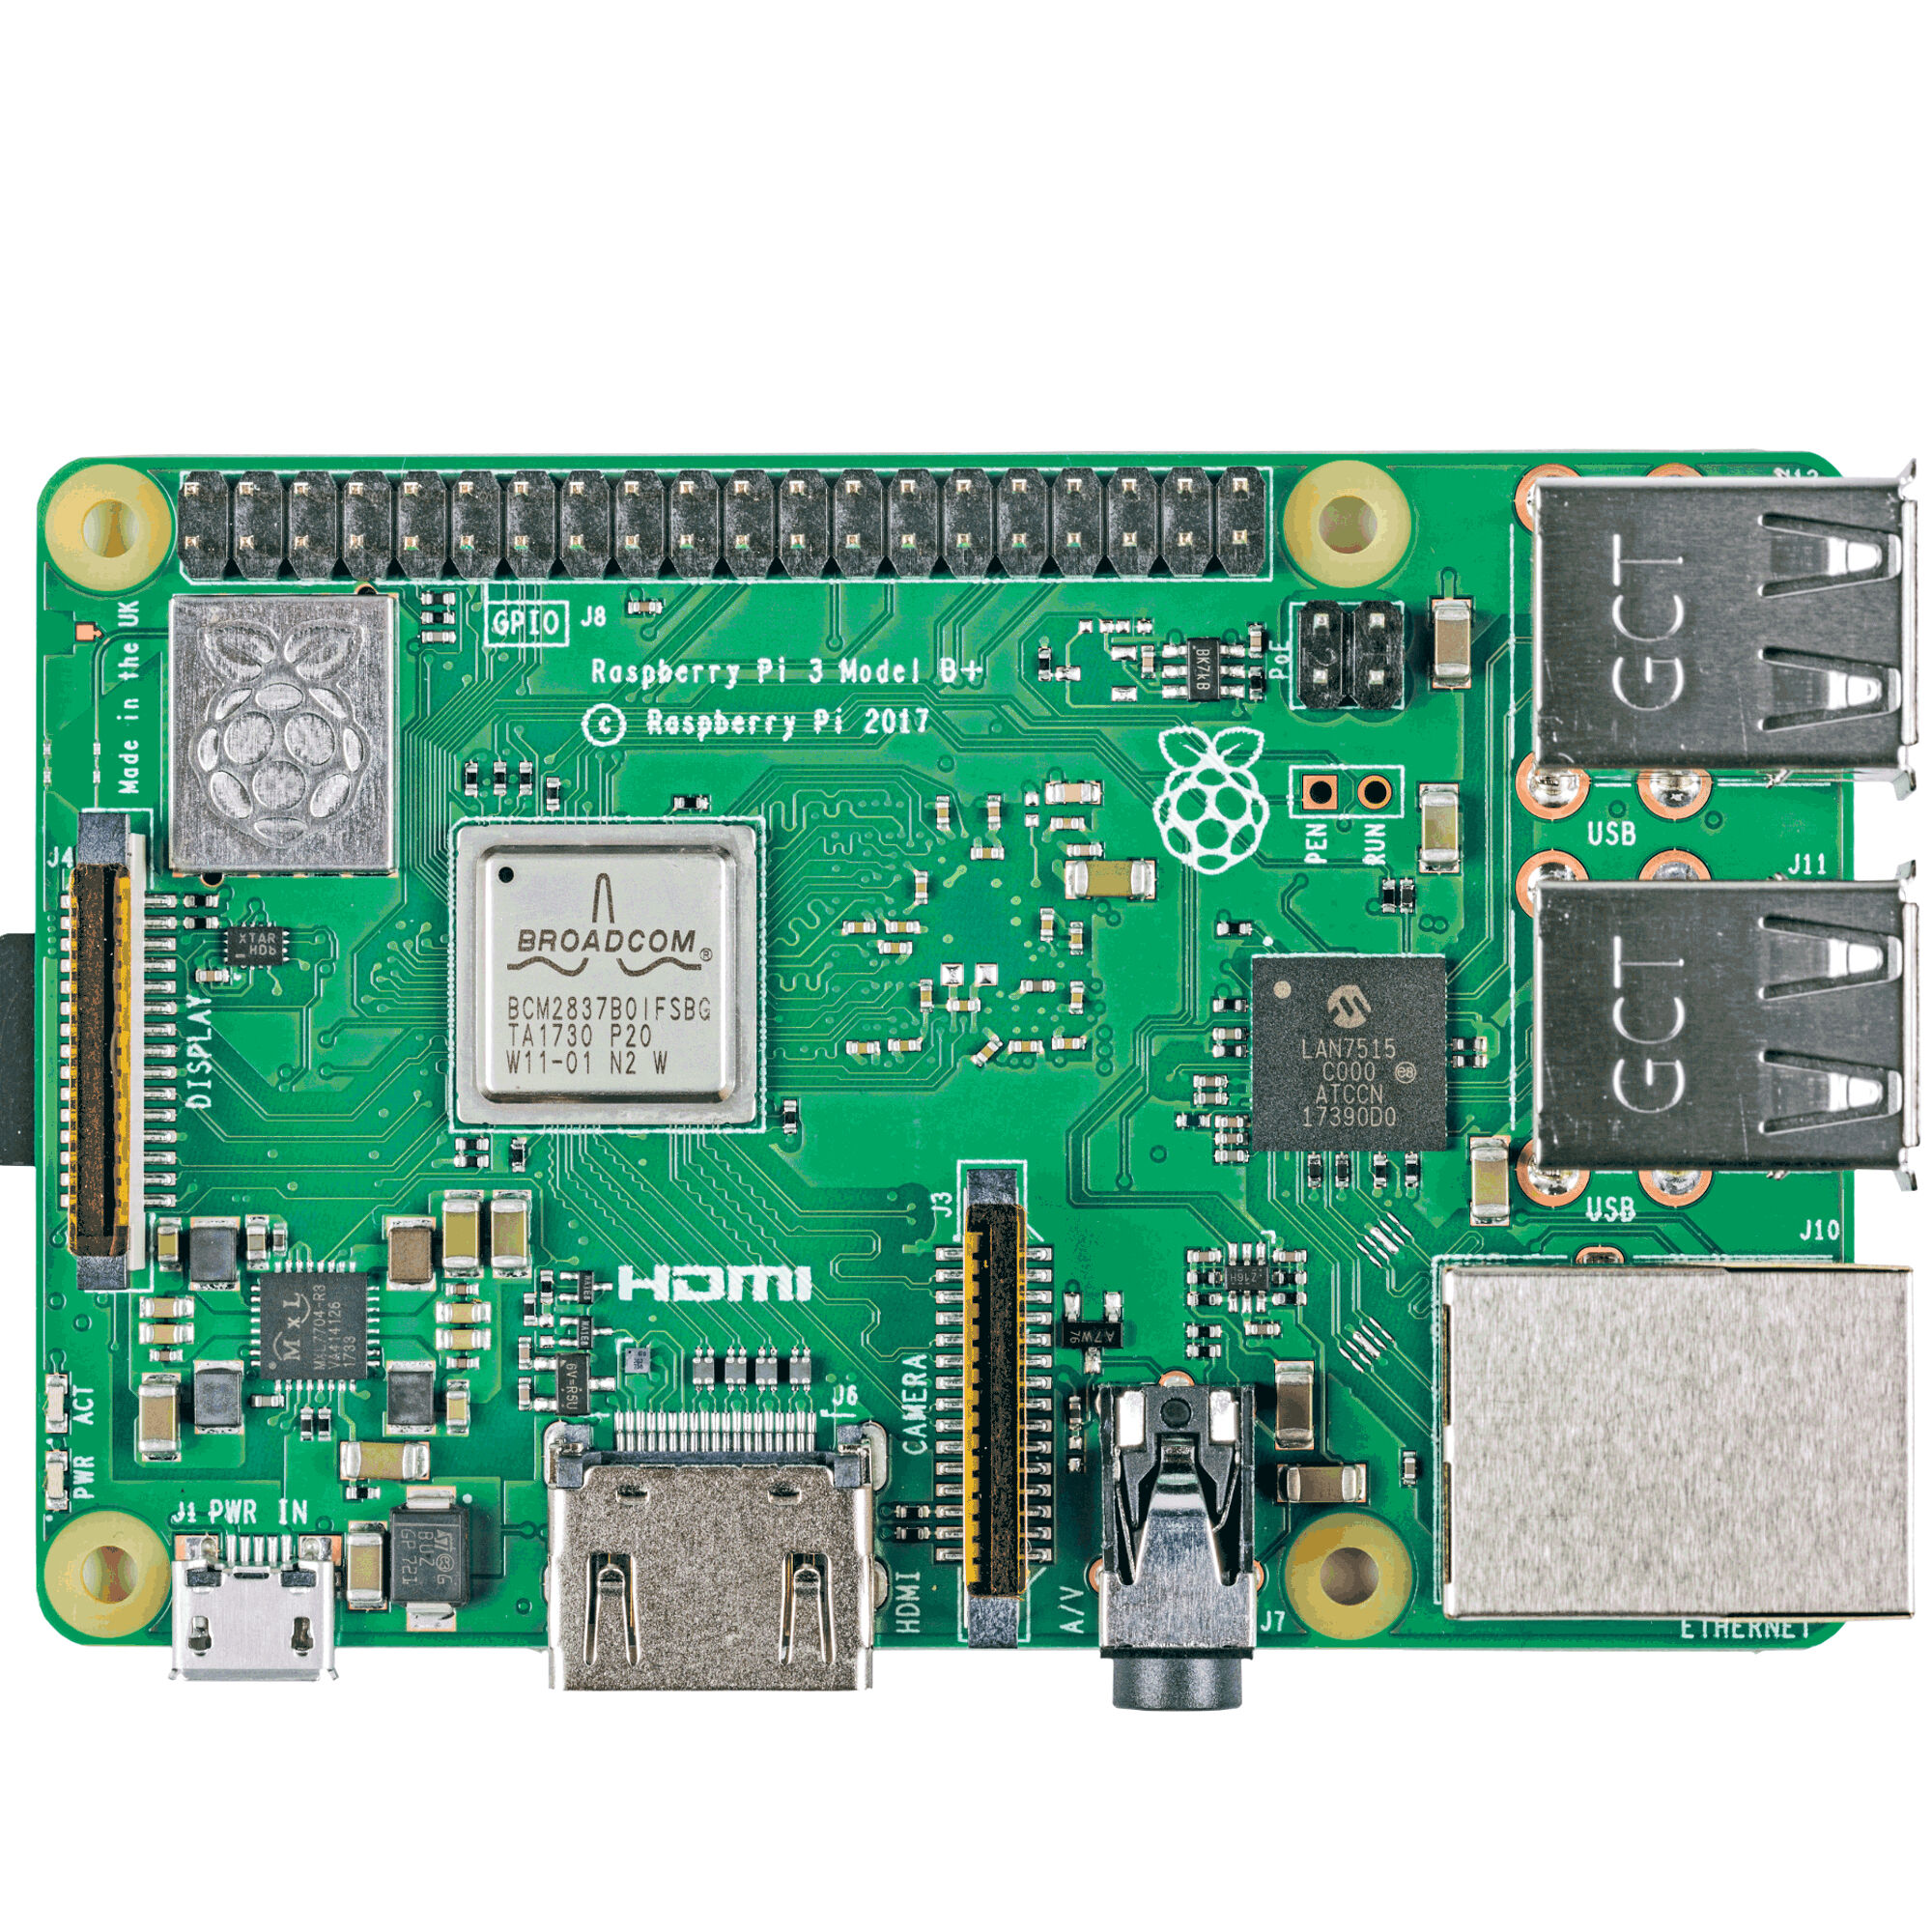
\includegraphics[width=0.55\textwidth]{pictures/RasPi.png}
    \caption{Raspberry Pi 3B+ \autocite{rasPi}}
  \end{figure}
\end{frame}

\begin{frame}[fragile]{CO$_2$-Sensor}
  \begin{figure}
    \centering
    \captionsetup{justification=centering}
    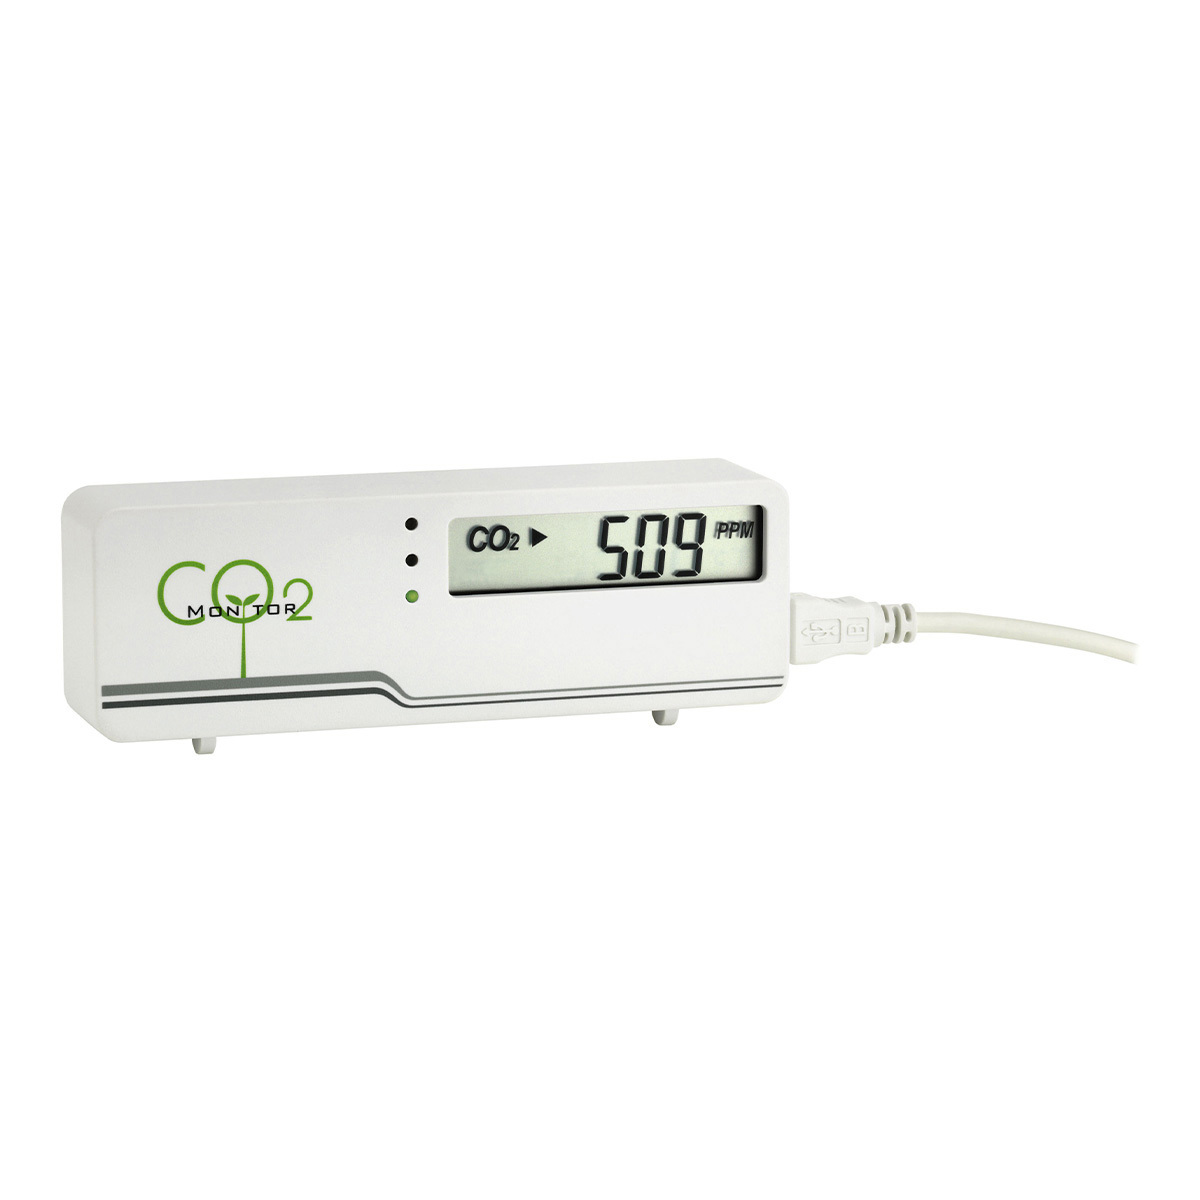
\includegraphics[trim={0 10cm 0 10cm},clip,width=0.85\textwidth]{pictures/co2monitor.png}
    \caption{TFA Dostmann AIRCO2NTROL MINI \autocite{co2monitor}}
  \end{figure}
\end{frame}


\section{Softwaretechnische Umsetzung}

\subsection{Grundlagen}
\begin{frame}[fragile]{Grundlagen}
  \begin{minipage}[t]{0.49\textwidth}
    \begin{itemize}
      \item Linux-Distribution inklusive mitgelieferter Standardsoftware
      \item Docker
      \item Python
      \item FastAPI
      \item React
      \item ChartJs
      \item SQLite
    \end{itemize}
  \end{minipage}
  \begin{minipage}[t]{0.49\textwidth}
    \begin{figure}
      \centering
      \captionsetup{justification=centering}
      
\includegraphics[width=1\textwidth]{pictures/SoftwareKomponenten.png}
      \caption{Verwendete Softwarekomponenten \autocite{dockerLogo}\autocite{fastapiLogo}\autocite{sqliteLogo}\autocite{reactLogo}\autocite{pythonLogo}\autocite{chartjsLogo}}
    \end{figure}
  \end{minipage}
\end{frame}

\subsection{Zusammenspiel der Softwarekomponenten}

\begin{frame}[fragile]{Zusammenspiel der Softwarekomponenten}
  \begin{figure}
    \centering
    \captionsetup{justification=centering}
    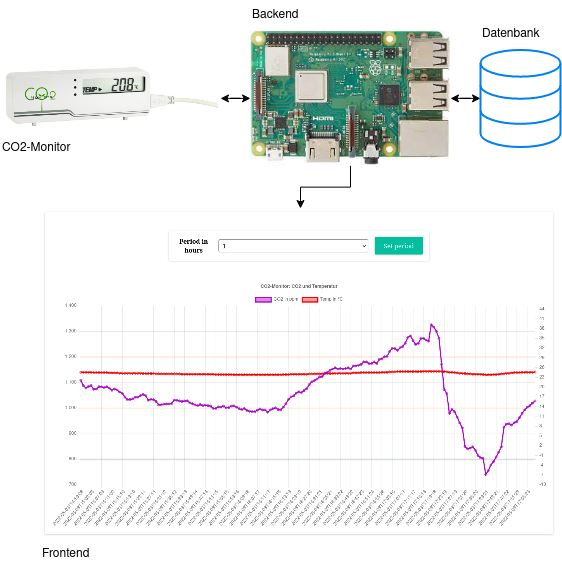
\includegraphics[width=0.6\textwidth]{pictures/SoftwareZusammenspiel.png}
    \caption{Zusammenspiel der Softwarekomponenten \autocite{co2monitor}\autocite{rasPi}}
  \end{figure}
\end{frame}

\subsection{Aufbau und Einrichtung der Softwarekomponenten}

\begin{frame}[fragile]{Aufbau und Einrichtung der Softwarekomponenten}

  \begin{minipage}[t]{0.49\textwidth}
    \begin{itemize}
      \item Backend: Python mit FastAPI
      \item Frontend: React und ChartsJs
      \item Lese-Software: Python-Script
      \item Datenbank: SQLite
    \end{itemize}
  \end{minipage}

  \begin{lstlisting}[language=Bash]
    docker-compose -f docker-compose.yml up -d
  \end{lstlisting}
\end{frame}

\section{Fazit}
\begin{frame}[fragile]{Fazit}
  \begin{minipage}[t]{0.80\textwidth}
    \textbf{Ergebnisse:}\newline
    \begin{itemize}
      \item bestätigte Relevanz der Raumluftqualität
      \item bestätigte Verbindung zwischen hohen CO$_2$-Konzentrationen und verminderter Konzentrationsfähigkeit/Produktivität
      \item schaffen einer kostengünstigen Möglichkeit zur selbstständigen Kontrolle der Raumluftqualität
    \end{itemize}
  \end{minipage}
\end{frame}

\begin{frame}[standout]
  Fragen?
\end{frame}

\appendix

\begin{frame}[allowframebreaks]{Literaturverzeichnis}

  \printbibliography[title={Quellenverzeichnis}]

\end{frame}

\begin{frame}[standout]
  Danke für die Aufmerksamkeit!
\end{frame}
\end{document}
